%%%%%%%%%%%%%%%%%%%%%%%%%%%%%%%%%%%%%%%%%%%%%%%%%%%%%%%%%%%%%%%%%%%%%%%
%%%%  Load the document class and packages                         %%%%
%%%%%%%%%%%%%%%%%%%%%%%%%%%%%%%%%%%%%%%%%%%%%%%%%%%%%%%%%%%%%%%%%%%%%%%
\documentclass[a4paper]{report}
\usepackage{epsfig}            % to insert PostScript figures
\graphicspath{
	{./figures/}
}

%Change figure names
\renewcommand{\figurename}{Fig}

\usepackage[bf,footnotesize]{caption} % make captions small and label bold

\addtocounter{chapter}{1} %Because starting at zero is silly
\makeatletter
\renewcommand{\thesection}{\@arabic\c@section}
\renewcommand{\thefigure}{\@arabic\c@figure}
\makeatother

\usepackage{titlesec} %change spacing before and after sections
%format: \titlespacing*{<command>}{<left>}{<before-sep>}{<after-sep>}
\titlespacing*{\section}{0pt}{11mm plus 1ex minus .2ex}{6mm plus .2ex}
\titlespacing*{\subsection}{0pt}{9mm plus 1ex minus .2ex}{4mm plus .2ex}

\usepackage[a4paper,margin=3.7cm,tmargin=2.5cm,bmargin=2.5cm]{geometry}
\usepackage{textcomp}  % To make nice degree symbols and others
\usepackage[bf,footnotesize]{caption} % make captions small and label bold
\usepackage{wrapfig}
%to produce the clickable references along the left in Acroread. This
%package must be included last.
\usepackage[ps2pdf,bookmarks=TRUE]{hyperref}
\hypersetup{
    colorlinks=true,
    linkcolor=cyan,
    filecolor=magenta,
    urlcolor=cyan,
}
\usepackage{wrapfig}

%%%%%%%%%%%%%%%%%%%%%%%%%%%%%%%%%%%%%%%%%%%%%%%%%%%%%%%%%%%%%%%%%%%%%%%
%%%%  Hypertext references for Acrobat                             %%%%
%%%%%%%%%%%%%%%%%%%%%%%%%%%%%%%%%%%%%%%%%%%%%%%%%%%%%%%%%%%%%%%%%%%%%%%
\hypersetup{
	pdfauthor = {SWC},
	pdftitle = {Optics Exercises},
	pdfkeywords = {optics, lenses, refraction, reflection, dispersion,
		telescope, microscope},
	pdfcreator = {LaTeX with hyperref},
	pdfproducer = {dvips + ps2pdf}
}

%%%%%%%%%%%%%%%%%%%%%%%%%%%%%%%%%%%%%%%%%%%%%%%%%%%%%%%%%%%%%%%%%%%%%%%
%%%%  Main text                                                    %%%%
%%%%%%%%%%%%%%%%%%%%%%%%%%%%%%%%%%%%%%%%%%%%%%%%%%%%%%%%%%%%%%%%%%%%%%%
\begin{document}

	%set the number of sectioning levels
	\setcounter{secnumdepth}{2}

	\begin{center}
		\textbf{\Large{Image Formation}}
	\end{center}

	%%%%%%%%%%%%%%%%%%%%%%%%%%%%%%%%%%%%%%%%%%%%%%%%%%%%%%%%%%%%%%%%%%%%%%%
%	\section{Introduction}
	%%%%%%%%%%%%%%%%%%%%%%%%%%%%%%%%%%%%%%%%%%%%%%%%%%%%%%%%%%%%%%%%%%%%%%%
	\vspace{0.8cm}
	\noindent The goal of this series of exercises is to gain an intuition of what lenses do and how they can be combined on a simple optical setup.

% 	\begin{itemize}
% 	    \item Bullet points are things to do
% 	    \item Hints are at the end of the document. Click on `Go to hint' and `Go back' to navigate. Don't just read the hint right away, but be sure to read it before moving on.
% 	    \item Help with the assembly of optics parts can be found in `Assembly Instructions'.
% 	\end{itemize}

%     current ToDos \\
%   - add phone pixel size question?
%   - add wavefront sensor question
% 	- add justification of thin lens approximation, paraxial rays etc.? \\
% 	- this goes into abberrations, where to treat them? just leave it to the lecture? \\
% 	- make assembly pics and put in 'General Instruction' \\
% 	- figure out laser pointer alignment problem \\
% 	- finish hint for telescope \\
% 	- finish hints for challenge questions \\
% 	- add question with sensor size? use basler acA1440-220um vs. acA2040-120um


    %%%%%%%%%%%%%%%%%%%%%%%%%%%%%%%%%%%%%%%%%%%%%%%%%%%%%%%%%%%%%%%%%%%%%%%
	\section{Image formation -- quick recap}
	%%%%%%%%%%%%%%%%%%%%%%%%%%%%%%%%%%%%%%%%%%%%%%%%%%%%%%%%%%%%%%%%%%%%%%%
	\hypertarget{hintBack-recap}{}

     Figure~\ref{fig:raytracerules} illustrates the three rules of ray-tracing through an ideal convex (positive) lens.
     By definition, convex lenses focus parallel rays to a spot at a distance of 1 focal length from the lens.
     The is illustrated by rules A and B, which are equivalent (B is the reverse of A).
     Rule C shows the special case where the angle of the ray leaving the lens is the same as the angle of the ray entering the lens.


	\begin{figure}[h]
		\center
		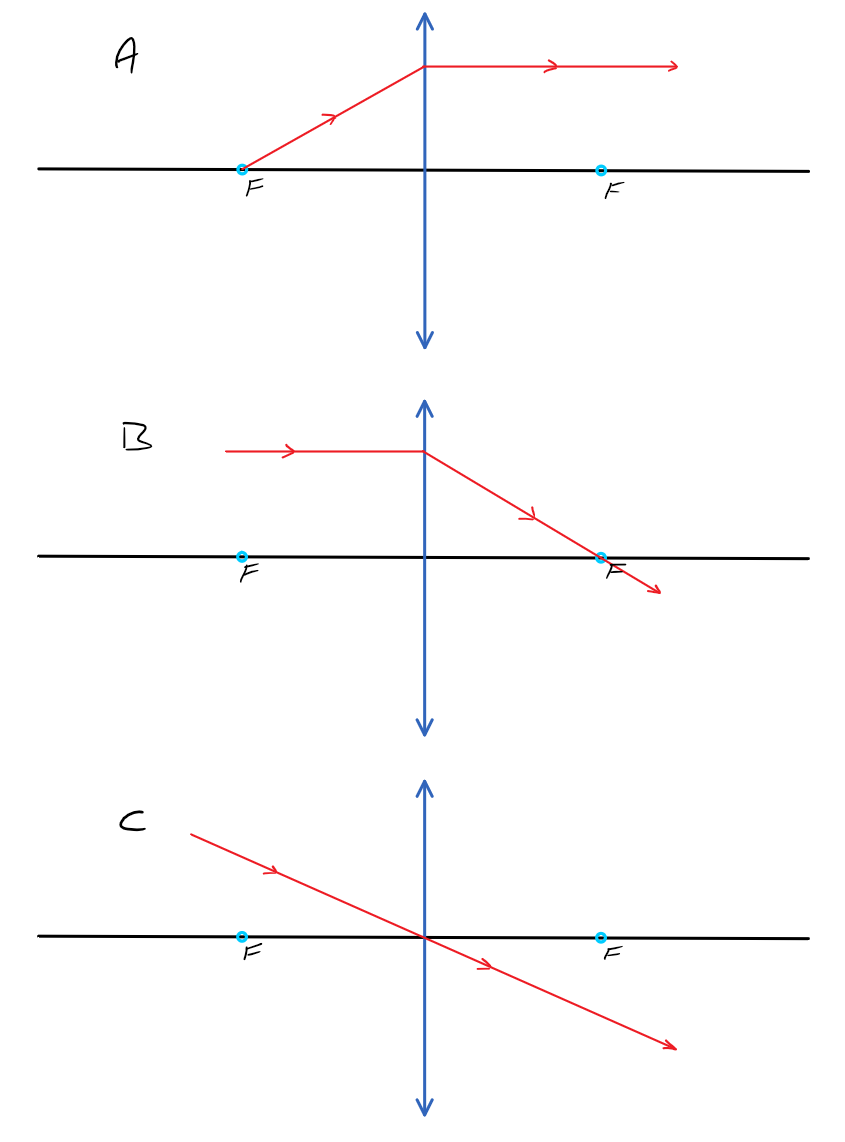
\includegraphics[width=0.8\textwidth]{figures/ray_trace_rules.png}
		\captionsetup{width=0.95\textwidth}
		\caption{The three rules of ray-tracing through a thin convex lens.
		\textbf{A}. Rays (red) originating from the front focal point exit the lens parallel to the optical axis (black line).
		\textbf{B}. Rays entering the lens parallel to the optical axis will pass through the rear focal point.
		\textbf{C}. Rays traveling through the centre of the lens are not deviated: leaving the lens at the same angle at which they entered it.
		}
		\label{fig:raytracerules}
	\end{figure}

	\clearpage

	\textbf{An image is formed when light rays leaving one point of an object converge again at another point in space}.
	This is illustrated in Fig.~\ref{fig:imageforming}, where the penguins on the left are imaged through an idealised thin lens.
	Two of the privileged rays from Fig.~\ref{fig:raytracerules} are shown for each penguin object:
	\begin{itemize}
	\item The color-coded rays correspond to the undeviated case shown in Fig.~\ref{fig:raytracerules}C.
	\item The exiting black ray corresponds to Fig.~\ref{fig:raytracerules}B: it enters the lens parallel to the optical axis and gets refracted to the focal point.
	\end{itemize}
	Note how all penguins share the second, parallel, ray -- it thus becomes easily apparent how the image-forming condition varies according to the angle of the centre ray.

	\begin{figure}[h]
		\center
		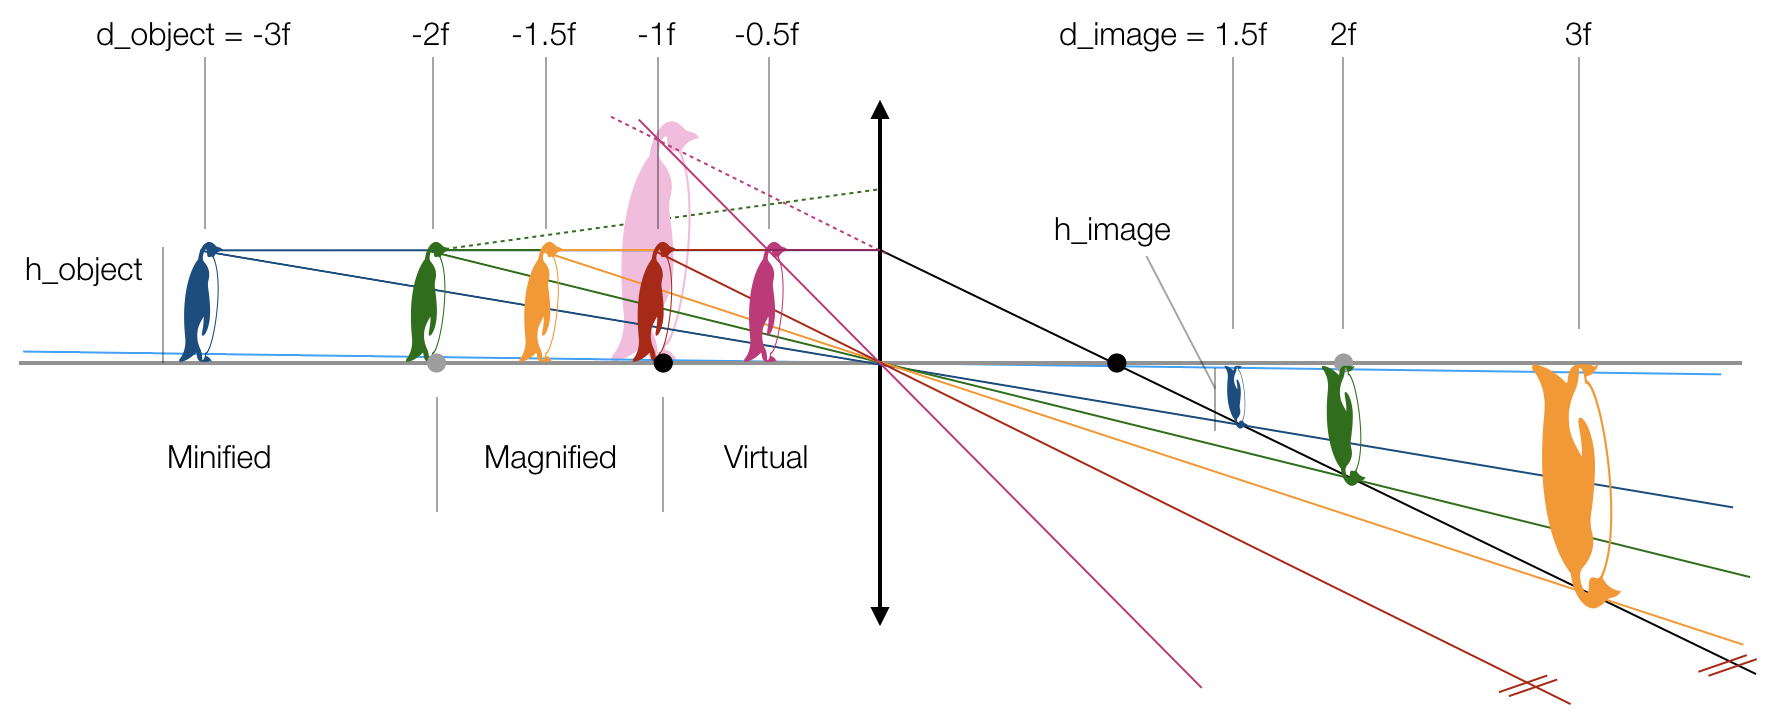
\includegraphics[width=1\textwidth]{figures/penguin_lens.png}
		\captionsetup{width=0.95\textwidth}
		\caption{Image formation using an idealised thin lens with focal length $f$. Object and image distance are shown in function of $f$.
		The light blue ray close to the optical axis illustrates how, for $d_o$ close to infinity, the image will be formed ever closer to the focal point (this ray comes from a very distant penguin's beak).
		}
		\label{fig:imageforming}
	\end{figure}

	\noindent
	   The distance at which the image forms is given by the thin lens equation (note that $d_o$ is negative):
	\begin{equation}
	\frac{1}{f} = \frac{1}{d_i} - \frac{1}{d_o}
	\label{eq:thinlens}
	\end{equation}

	Sign conventions follow Cartesian coordinates (objects placed to the left of the lens are at negative distances). For positive (convex) lenses, $f>0$. For negative (concave) lenses, $f<0$.

	\begin{itemize}
	    \item Convince yourself that the thin lens equation matches the ray tracing
	    \item All rays, not just the `privileged rays' (Fig.~\ref{fig:raytracerules}), leaving a point on the penguin's head and passing through an ideal lens will meet again in the image plane. Using a `helper ray` confirm that the green dotted ray leaving the green penguin's head in Fig.~\ref{fig:imageforming} will indeed converge with the others in the image plane.
	\end{itemize}


    \clearpage

	%%%%%%%%%%%%%%%%%%%%%%%%%%%%%%%%%%%%%%%%%%%%%%%%%%%%%%%%%%%%%%%%%%%%%%%
	\section{Please meet the lens}
	%%%%%%%%%%%%%%%%%%%%%%%%%%%%%%%%%%%%%%%%%%%%%%%%%%%%%%%%%%%%%%%%%%%%%%%

	%----------------------------------------------------------------------
    \subsection{Determine the focal length of a convex lens}
    %----------------------------------------------------------------------
	\hypertarget{hintBack-focal_length}{}
	Your optics kit contains a number of small plastic boxes, each containing a lens whose focal length may or may not match what is printed on its box.
	How can you estimate the focal length of a lens and thereby determine whether it matches what is stated on the box?
    There are a couple of easy ways this can be done using only the lens in question.



	%----------------------------------------------------------------------
    \subsection{Forming an image with a lens}
    %----------------------------------------------------------------------
	\hypertarget{hintBack-image}{}
	As you are reading this, the lenses in your eyes are forming images of the text onto the retina.
	In the room, we don't have a closed space like the eye to shield the detector from stray light, making it hard to see images of the room formed by a lens onto a piece of paper (stray light reduces \emph{contrast}).
	So we will use a bright LED as an object -- this will allow us to see the image of the LED emitter formed on a piece of paper.

	\subsubsection{Setting up the LED}
	Your first task is to set up the LED on the optical rail (make sure you have first read the `Assembly Hints'):
	\begin{itemize}
    \item Attach a post holder to a rail carriage and place this on the rail.
    \item Attach a 50 mm post to the white LED glued to a cage plate and place this in the post holder.
    \item Power the LED using the ThorLabs LED driver and LED power cable.
	\end{itemize}

	\subsubsection{Forming an image of the LED emitter}
	Choose any lens and mount it in a lens holder using the lens tool.
	Mount the lens on the rail with a second carriage, post, and post holder.
	You can form an image of the LED emitter on a white card or you can use the plastic post-mountable screen.

    \begin{itemize}
	    \item How do you expect image size, location, and magnification to vary with object distance (refer to Fig.~\ref{fig:imageforming})? Verify that these are true by forming images of the LED emitter on the card for different values of $d_o$. (The LED emitter looks like a small square with dots in a grid -- if all you see is a blur, you are not looking at an image)
	    \item Under what circumstances will you \emph{not} form an image of the emitter? Draw the ray diagram and try it on the rail.
	    \item The magnification of the object in the image plane is given by  $m = h_i / h_o = d_i / d_o$. $m=1$ indicates unitary magnification. Negative indicates an inverted image.
	Use the optical setup to measure the true size of the LED emitter.
	\end{itemize}

    \clearpage

	\subsubsection{Forming an image of a distant source}
    Use a lens of about $f=60~mm$ to form an image of the room lights on a piece of paper.
    The image will be formed at very close to $1f$.
    Repeat with a lens of about $f=200~mm$.
    What two things do you notice about the images produced by these lenses?
    Fig.~\ref{fig:outside} models the situation you saw.
    Can you explain your observations using these ray diagrams?


    \begin{figure}[h]
    \center
    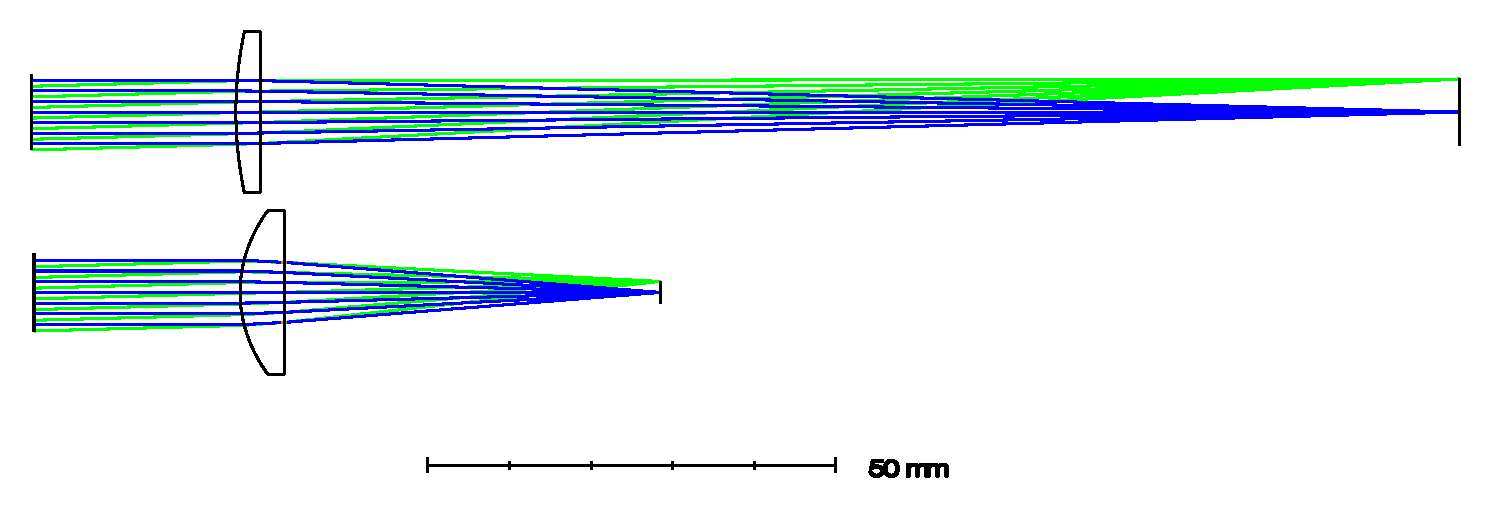
\includegraphics[width=6in]{figures/lens_f_comparison.eps}
    \caption{Images formed at $1f$ from light originating at infinity.
    The top is a $f=150~mm$ lens and the bottom a $f=50~mm$ lens.
    Light from different regions of the object arrive in parallel rays that come in at different angles (green and blue).
    Each set of parallel rays come into focus at a point, satisfying the image-forming condition. }
    \label{fig:outside}
    \end{figure}


	%----------------------------------------------------------------------
    \subsection{Virtual images}
    %----------------------------------------------------------------------
    \hypertarget{hintBack-virtual}{}
    The images you have formed above are \emph{real images}, meaning that they are created by rays which are \emph{converging}.
    In other words, a real image is a collection of focus points that is created by converging rays.
    A \emph{virtual image}, on the other hand, is composed of a collection of points whose rays are \emph{diverging}.
    Unlike real images, virtual images can not be projected onto a screen and require an additional lens in order to achieve this.

    Figure~\ref{fig:mirror} shows how a flat mirror forms a virtual image of an object apparently positioned behind the mirror.
    The rays seem to diverge from points behind the mirror and the image is not magnified: the object appears to be as far behind the mirror as the object is in front of the mirror.
    The image of the bottle is only formed once rays are converged by a positive lens and focused on to a screen (e.g. as in the observer's eye).

    \begin{figure}[h]
    \center
    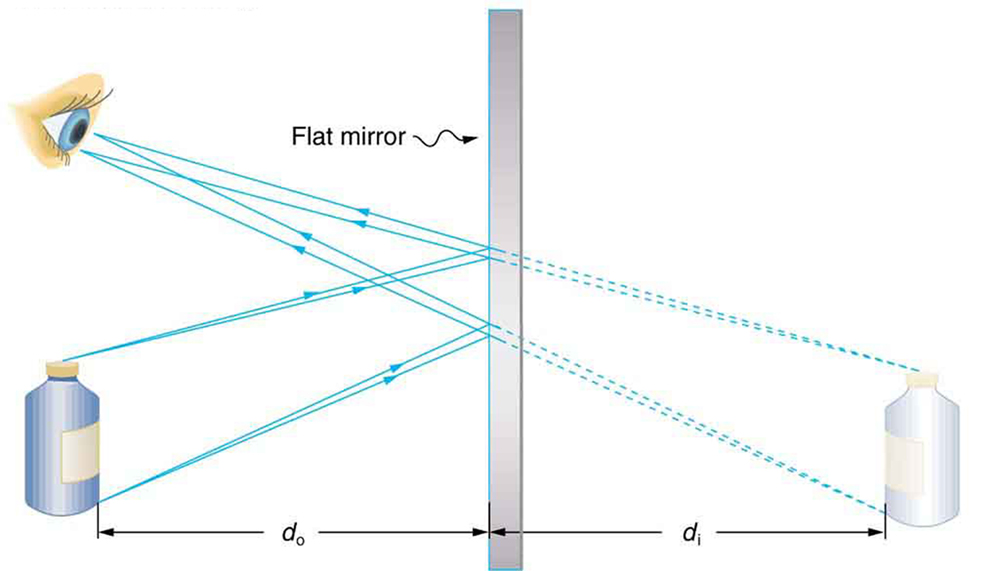
\includegraphics[width=4in]{figures/virtual_image_mirr.jpg}
    \caption{A virtual image of the bottle is created on the far side of the mirror.
    This is described by the dotted lines which are `extended rays' that are used to form the virtual image. }
    \label{fig:mirror}
    \end{figure}

    \clearpage

    Light rays from a virtual image are angled such that they \emph{appear} to emanate from a point in the virtual image plane, but they never actually met in that point.
    This is seen starkly in Fig.~\ref{fig:negative_lens_tracing}, which is the ray diagram for a negative (concave) lens.

    \begin{figure}[h]
		\center
		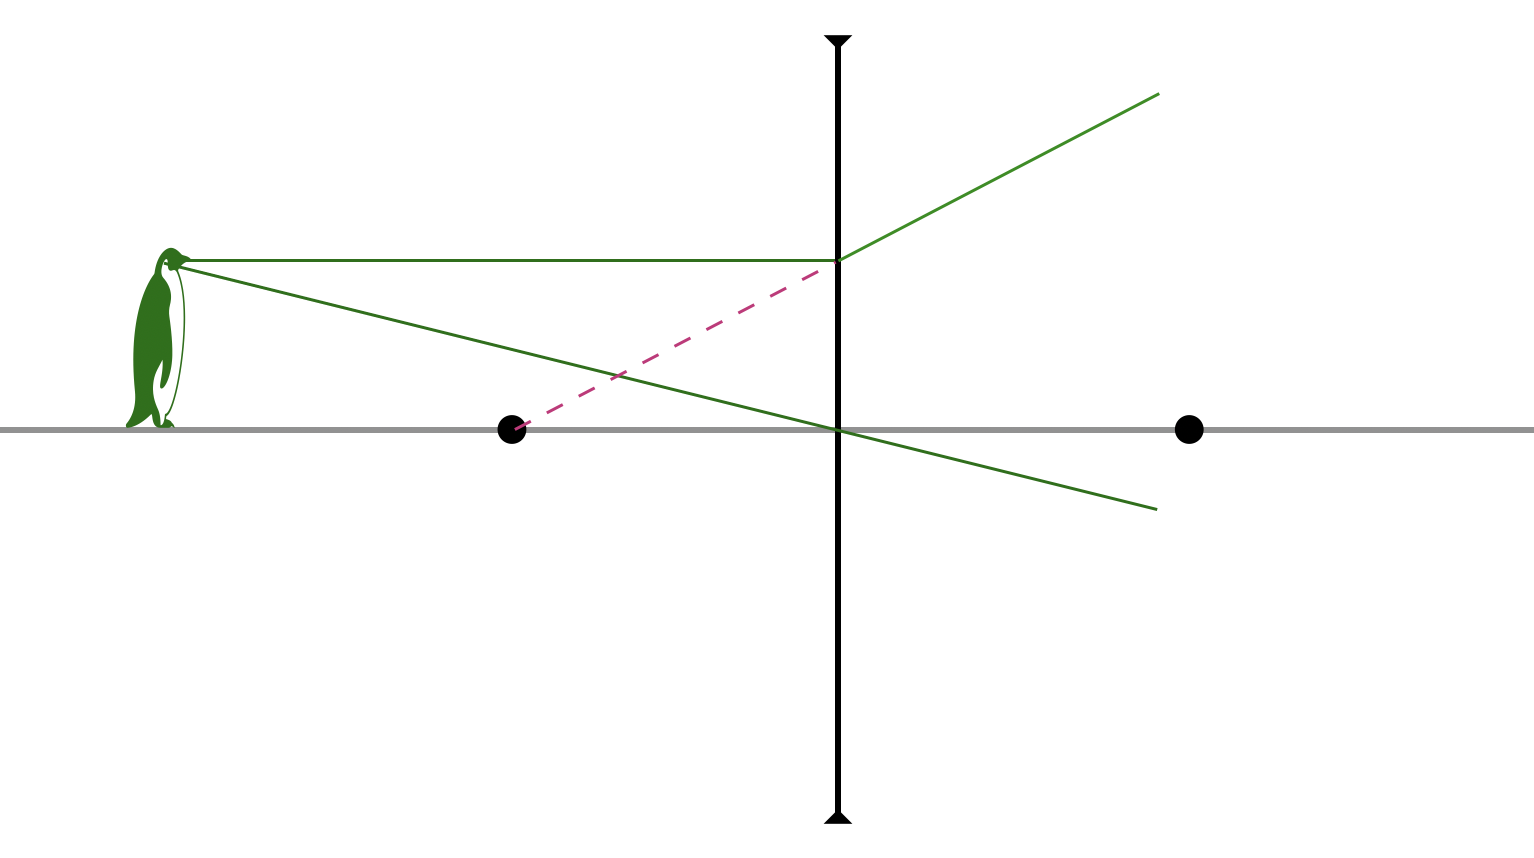
\includegraphics[width=0.5\textwidth]{figures/negative_lens_tracing.png}
		\captionsetup{width=0.6\textwidth}
		\caption{Ray tracing for a negative lens. The `identity' of the focal points is swapped compared to a positive lens -- the green ray parallel to the optical axis hits the lens and is drawn down to the focal point \emph{on the same (object) side}, as shown in dotted pink. This gives you the angle of the ray after the lens. \emph{Rays from the penguin's beak appears to emanate from the point where the dotted ray meets the ray going through the centre of the lens}.
		}
		\label{fig:negative_lens_tracing}
	\end{figure}

    \begin{itemize}
        \item Can you form a virtual image with a positive (convex) lens? If so, draw the ray diagram.
        \item Check this with your own eyes (look through the lens at an object). Is this configuration ever used in daily life?
        \item Imagine (draw) what you see for $d_0$ close to $f$? See if you are right.
        \item Can you tell whether a lens is negative (diverges parallel light) or positive (converges parallel light) without using light, just by looking at the shape?
        \item What will you see if you look through a negative (concave) lens? Draw a ray diagram (don't forget your eye as the second lens). Check your expectations with the $f=-50mm$ lens from your kit.
        \item You might find an unlabeled negative lens - how could you determine its focal length?
    \end{itemize}

    \clearpage


	%%%%%%%%%%%%%%%%%%%%%%%%%%%%%%%%%%%%%%%%%%%%%%%%%%%%%%%%%%%%%%%%%%%%%%%
	\section{Multiple lenses}
	%%%%%%%%%%%%%%%%%%%%%%%%%%%%%%%%%%%%%%%%%%%%%%%%%%%%%%%%%%%%%%%%%%%%%%%

	You have seen that a lot can be done with a single lens: it can form images of different magnification and even create virtual images.
	However, the real power of optical systems only becomes apparent when we chain together sequences of lenses.
	In this scenario the image created by an upstream lens acts as the object to be imaged by a downstream lens.
	We will now examine two important scenarios that arise from pairs of lenses: the \emph{finite conjugate} configuration and the \emph{infinite conjugate} configuration.
	\textbf{You will encounter these configurations again and again throughout the course}.

	%----------------------------------------------------------------------
	\subsection{Infinite conjugate configuration}
	%----------------------------------------------------------------------
	\hypertarget{hintBack-infinite}{}

	Let's begin with the `infinite conjugate', which is built using two lenses.
	The term `conjugate' refers to the correspondence between the object and image planes.
	The term `infinite' indicates that the lens forming the image does so with an object located at infinity.
	Thus, the object conjugated with the image is at infinity.

	\begin{itemize}
		\item Draw a ray diagram of two lenses with $f_1=2 \cdot f_2$, $f_1$ apart. The object should be at $-f_1$ of the first lens. Where does the image form?
		\item Increase the distance between the lenses to $2\cdot f_1$ and redraw (or use another color on the same drawing), using the ray tracing rules. Where does the image form now? What happened to the magnification?
		\item What is the magnification of the image? Deduce the formula using similar triangles in your ray diagram.
		\item What could be the use of such a two-lens system in infinite conjugate configuration?
	\end{itemize}

    \noindent
	Let's verify your predictions on the rail with two lenses of your choice.

	\begin{itemize}
	    \item First, ensure the first lens is at $f_1$ from the LED (the object) before placing the second lens. You could use a ruler, but it can be hard to know where to measure from (where the optical centre of your lens is). What is a smarter way of doing it?
	    \item Place the second lens, and find where the image forms.
	    \item Verify the infinite space by moving the second lens and finding again with the screen where the image forms. Are your expectations met?
	\end{itemize}




	%----------------------------------------------------------------------
	\subsection{Beam expanders}
	%----------------------------------------------------------------------
	\hypertarget{hintBack-expand}{}

	Lasers are wonderful devices that produce light that is \emph{collimated}, or parallel. The idealised depiction is a beam of a certain width that stays parallel (in reality, they always expand / diverge to some degree). Before the invention of lasers in 1960, microscopy was much worse off.

    \begin{itemize}
        \item Can you collimate your LED? Draw the ray diagram.
		\item For reasons discussed later, the diameter of a laser beam in an optical system may need to be adjusted. Come up with a way to change the width of a collimated laser beam -- draw the ray diagram. What determines the size change? Deduce a formula from your diagram.
	    \item Can you accomplish the task using a positive and a negative lens?
	\end{itemize}

    \noindent
	To build the beam expander on the rail, we will i) align the laser diode to the rail using an iris, and ii) align the lenses with respect to the aligned beam.


    \noindent
	Aligning the laser to the rail:
	\begin{itemize}
	    \item Check the `Assembly Instructions' to set up the rail, laser and iris.
	    \item Understand and implement the procedure depicted in Fig. \ref{fig:laser_alignment}. Iterate between the close and far position until the beam is straight.
	\end{itemize}


	\begin{figure}[h]
		\center
		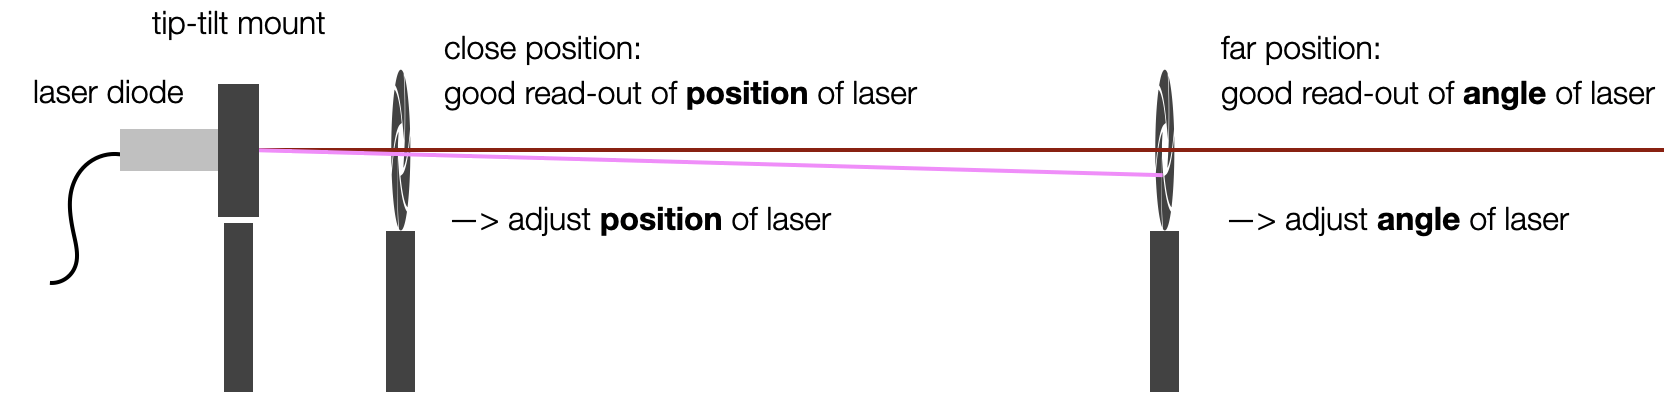
\includegraphics[width=0.9\textwidth]{figures/laser_alignment.png}
		\captionsetup{width=0.9\textwidth}
		\caption{Aligning the laser using a translating iris on the rail. When the iris is up against the laser, the angle of the beam changes little where it hits the iris -- but the height and lateral position matter a lot. Conversely, when the iris is far away, the angle of the beam matters most. Thus, the iris in close position allows you to find the correct position in space of the laser that intersects the imaginary line passing through the irises; the iris in far position allows you to find the correct angle of the beam.}
		\label{fig:laser_alignment}
	\end{figure}

	\noindent
	Placing of the beam expander:
	\begin{itemize}
	    \item \textbf{Coarse alignement:} First align by eye as best as you can -- all optical elements should be placed straight and centred at the same height. Use a ruler to ensure approximate distance between lenses is correct.
		\item \textbf{Fine alignment:} The lens is at the correct height if the beam still hits the iris centred after the lens is in place (assuming the laser is aligned!). You can also look at the back reflection from the lens, which should go straight back to the laser if all is straight (use lens paper to see the beam path).
		\item How can you ensure the two lenses are $f_1+f_2$ apart?
        \item Build a beam expander to yield the maximum magnification your optics kit allows.
		\item The beam expander you have built also goes by another common name.  What is it?
		Think about what happens to beams that do not travel on-axis (Fig.~\ref{fig:telescope}). Once you've figured it out, remove the laser pointer, unfasten the rail and use your device.
	\end{itemize}



	\begin{figure}[h]
		\center
		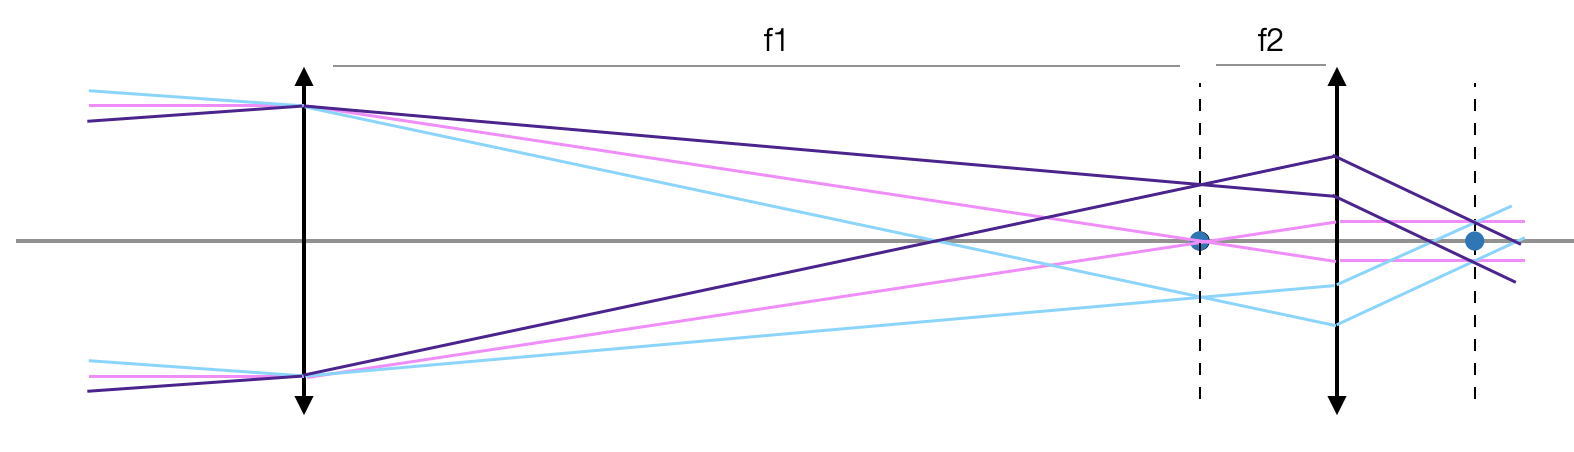
\includegraphics[width=0.9\textwidth]{figures/telescope.png}
		\captionsetup{width=0.9\textwidth}
		\caption{A Beam expander. In addition to the collimated beam arriving on-axis (pink), two off-axis beams are shown in different colors. Note how the angles of the beams leaving the second lens are amplified.}
		\label{fig:telescope}
	\end{figure}

	\clearpage

	%----------------------------------------------------------------------
    \subsection{Four lenses challenge}
    %----------------------------------------------------------------------
	Arrange 4 lenses, one of which must be a negative lens, so as to form a de-magnified, real, upright image.
	Reason through it, and remember that the image formed by the first lens is the object for the second, and so on. Pointers:
	\begin{itemize}
    	\item For an object, use a glass slide with an arrow painted on the frosty label end. Collimate your LED first to get as much light from it as possible - a lot will be lost along the way. Illuminate the arrow from behind.
		\item Space will be a problem: the lenses will take up the whole rail and so you will need to place the target and screen outside of the rail.
		\item Do coarse alignment - look at your setup from the side / top and ensure all optical elements are centered with respect to each other
		\item There are multiple solutions to this problem.
	\end{itemize}

\end{document}
